\documentclass[border=5mm]{standalone}
\usepackage[utf8]{inputenc}
\usepackage[T1]{fontenc}
\usepackage{amsmath}
\usepackage{tikz}
\usepackage{pgfplots}
\pgfplotsset{compat=1.18}
\usetikzlibrary{arrows.meta}
\definecolor{utnblue}{RGB}{0, 51, 102}

% Ej8 zonas: x(τ)=1 en [0,1] (pulso), h(t-τ)=(t-τ) en [t-2, t] (rampa invertida)
% 5 zonas: I (t<0), II (0≤t≤1), III (1<t≤2), IV (2<t≤3), V (t>3)
% Paneles I-IV. Misma escala (cm/unidad) que fig_ej8_signals.

\begin{document}
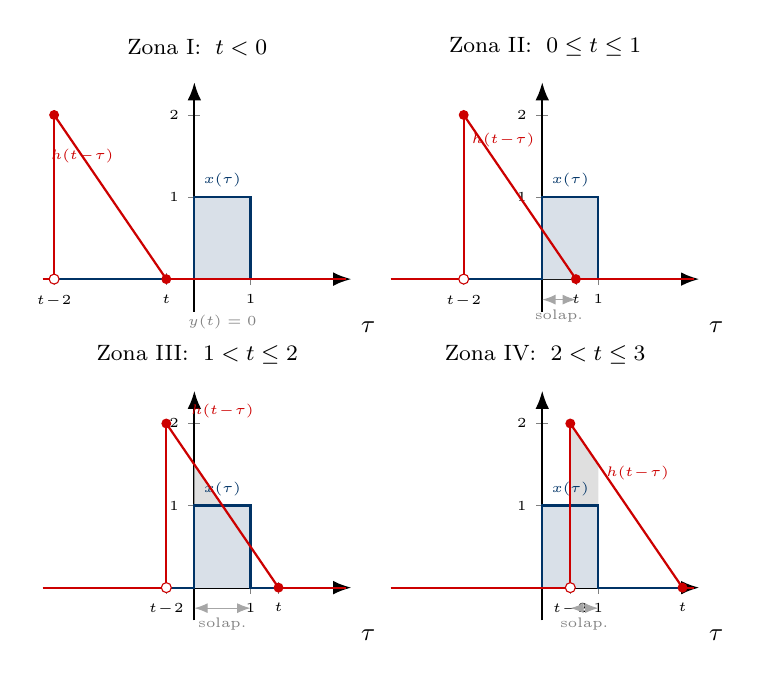
\begin{tikzpicture}[>=Latex, font=\small]

\colorlet{xcol}{utnblue}
\colorlet{hcol}{red!80!black}

\pgfmathsetmacro{\tmin}{-2.7}
\pgfmathsetmacro{\tmax}{2.8}

% =====================================================================
% ZONA I: t = -0.5 (sin solapamiento)
% =====================================================================
\begin{axis}[
    name=z1,
    width=5.5cm, height=4.5cm,
    axis lines=center,
    xlabel={$\tau$},
    xlabel style={anchor=north west, at={(axis description cs:1,0)}},
    xmin=\tmin, xmax=\tmax,
    ymin=-0.4, ymax=2.4,
    clip=false,
    axis line style={->, thick},
    xtick={-2.5,-0.5,0,1},
    xticklabels={$t\!-\!2$,$t$,$0$,$1$},
    ytick={0,1,2},
    every tick label/.style={font=\tiny},
    title={\footnotesize Zona~I:\; $t < 0$},
]
    % x(τ): pulso [0,1]
    \fill[xcol!15] (axis cs:0,0) rectangle (axis cs:1,1);
    \draw[xcol, thick]
        (axis cs:\tmin,0) -- (axis cs:0,0) -- (axis cs:0,1)
        -- (axis cs:1,1) -- (axis cs:1,0) -- (axis cs:{\tmax-0.1},0);
    \node[xcol, font=\tiny, above] at (axis cs:0.5,1) {$x(\tau)$};

    % h(t-τ) con t=-0.5: cero a izquierda, rampa en [-2.5,-0.5], cero a derecha
    \addplot[hcol, thick, domain=\tmin:-2.5, samples=2] {0};
    \addplot[hcol, thick, domain=-2.5:-0.5, samples=2] {-0.5-x};
    \addplot[hcol, thick, domain=-0.5:{\tmax-0.1}, samples=2] {0};
    \draw[hcol, thick] (axis cs:-2.5,0) -- (axis cs:-2.5,2);
    \fill[hcol]  (axis cs:-2.5,2) circle (1.8pt);
    \fill[white] (axis cs:-2.5,0) circle (1.8pt);
    \draw[hcol]  (axis cs:-2.5,0) circle (1.8pt);
    \fill[hcol]  (axis cs:-0.5,0) circle (1.8pt);
    \node[hcol, font=\tiny] at (axis cs:-2.0,1.5) {$h(t\!-\!\tau)$};

    \node[font=\tiny, gray, below] at (axis cs:0.5,-0.32) {$y(t)=0$};
\end{axis}

% =====================================================================
% ZONA II: t = 0.6 (solapamiento parcial [0, t])
% =====================================================================
\begin{axis}[
    name=z2,
    at={(z1.east)}, anchor=west, xshift=0.5cm,
    width=5.5cm, height=4.5cm,
    axis lines=center,
    xlabel={$\tau$},
    xlabel style={anchor=north west, at={(axis description cs:1,0)}},
    xmin=\tmin, xmax=\tmax,
    ymin=-0.4, ymax=2.4,
    clip=false,
    axis line style={->, thick},
    xtick={-1.4, 0, 0.6, 1},
    xticklabels={$t\!-\!2$, $0$, $t$, $1$},
    ytick={0,1,2},
    every tick label/.style={font=\tiny},
    title={\footnotesize Zona~II:\; $0 \leq t \leq 1$},
]
    % solapamiento [0, 0.6]
    \fill[gray!25] (axis cs:0,0) -- (axis cs:0,0.6) -- (axis cs:0.6,0) -- cycle;

    % x(τ): pulso [0,1]
    \fill[xcol!15] (axis cs:0,0) rectangle (axis cs:1,1);
    \draw[xcol, thick]
        (axis cs:\tmin,0) -- (axis cs:0,0) -- (axis cs:0,1)
        -- (axis cs:1,1) -- (axis cs:1,0) -- (axis cs:{\tmax-0.1},0);
    \node[xcol, font=\tiny, above] at (axis cs:0.5,1) {$x(\tau)$};

    % h(t-τ) con t=0.6: cero a izq, rampa en [-1.4,0.6], cero a der
    \addplot[hcol, thick, domain=\tmin:-1.4, samples=2] {0};
    \addplot[hcol, thick, domain=-1.4:0.6, samples=2] {0.6-x};
    \addplot[hcol, thick, domain=0.6:{\tmax-0.1}, samples=2] {0};
    \draw[hcol, thick] (axis cs:-1.4,0) -- (axis cs:-1.4,2);
    \fill[hcol]  (axis cs:-1.4,2) circle (1.8pt);
    \fill[white] (axis cs:-1.4,0) circle (1.8pt);
    \draw[hcol]  (axis cs:-1.4,0) circle (1.8pt);
    \fill[hcol]  (axis cs:0.6,0) circle (1.8pt);
    \node[hcol, font=\tiny] at (axis cs:-0.7,1.7) {$h(t\!-\!\tau)$};

    \draw[<->, gray!70, thin] (axis cs:0,-0.25) -- (axis cs:0.6,-0.25);
    \node[font=\tiny, gray, below] at (axis cs:0.3,-0.25) {solap.};
\end{axis}

% =====================================================================
% ZONA III: t = 1.5 (h cubre todo el pulso, solapamiento [0,1])
% =====================================================================
\begin{axis}[
    name=z3,
    at={(z1.south west)}, anchor=north west, yshift=-1cm,
    width=5.5cm, height=4.5cm,
    axis lines=center,
    xlabel={$\tau$},
    xlabel style={anchor=north west, at={(axis description cs:1,0)}},
    xmin=\tmin, xmax=\tmax,
    ymin=-0.4, ymax=2.4,
    clip=false,
    axis line style={->, thick},
    xtick={-0.5, 0, 1, 1.5},
    xticklabels={$t\!-\!2$, $0$, $1$, $t$},
    ytick={0,1,2},
    every tick label/.style={font=\tiny},
    title={\footnotesize Zona~III:\; $1 < t \leq 2$},
]
    % solapamiento [0, 1]
    \fill[gray!25] (axis cs:0,0) -- (axis cs:0,1.5) -- (axis cs:1,0.5) -- (axis cs:1,0) -- cycle;

    % x(τ): pulso [0,1]
    \fill[xcol!15] (axis cs:0,0) rectangle (axis cs:1,1);
    \draw[xcol, thick]
        (axis cs:\tmin,0) -- (axis cs:0,0) -- (axis cs:0,1)
        -- (axis cs:1,1) -- (axis cs:1,0) -- (axis cs:{\tmax-0.1},0);
    \node[xcol, font=\tiny, above] at (axis cs:0.5,1) {$x(\tau)$};

    % h(t-τ) con t=1.5: cero a izq, rampa en [-0.5,1.5], cero a der
    \addplot[hcol, thick, domain=\tmin:-0.5, samples=2] {0};
    \addplot[hcol, thick, domain=-0.5:1.5, samples=2] {1.5-x};
    \addplot[hcol, thick, domain=1.5:{\tmax-0.1}, samples=2] {0};
    \draw[hcol, thick] (axis cs:-0.5,0) -- (axis cs:-0.5,2);
    \fill[hcol]  (axis cs:-0.5,2) circle (1.8pt);
    \fill[white] (axis cs:-0.5,0) circle (1.8pt);
    \draw[hcol]  (axis cs:-0.5,0) circle (1.8pt);
    \fill[hcol]  (axis cs:1.5,0) circle (1.8pt);
    \node[hcol, font=\tiny] at (axis cs:0.5,2.15) {$h(t\!-\!\tau)$};

    \draw[<->, gray!70, thin] (axis cs:0,-0.25) -- (axis cs:1,-0.25);
    \node[font=\tiny, gray, below] at (axis cs:0.5,-0.25) {solap.};
\end{axis}

% =====================================================================
% ZONA IV: t = 2.5 (solapamiento parcial [t-2, 1]=[0.5,1])
% =====================================================================
\begin{axis}[
    name=z4,
    at={(z3.east)}, anchor=west, xshift=0.5cm,
    width=5.5cm, height=4.5cm,
    axis lines=center,
    xlabel={$\tau$},
    xlabel style={anchor=north west, at={(axis description cs:1,0)}},
    xmin=\tmin, xmax=\tmax,
    ymin=-0.4, ymax=2.4,
    clip=false,
    axis line style={->, thick},
    xtick={0, 0.5, 1, 2.5},
    xticklabels={$0$, $t\!-\!2$, $1$, $t$},
    ytick={0,1,2},
    every tick label/.style={font=\tiny},
    title={\footnotesize Zona~IV:\; $2 < t \leq 3$},
]
    % solapamiento [0.5, 1]
    \fill[gray!25] (axis cs:0.5,0) -- (axis cs:0.5,2) -- (axis cs:1,1.5) -- (axis cs:1,0) -- cycle;

    % x(τ): pulso [0,1]
    \fill[xcol!15] (axis cs:0,0) rectangle (axis cs:1,1);
    \draw[xcol, thick]
        (axis cs:\tmin,0) -- (axis cs:0,0) -- (axis cs:0,1)
        -- (axis cs:1,1) -- (axis cs:1,0) -- (axis cs:{\tmax-0.1},0);
    \node[xcol, font=\tiny, above] at (axis cs:0.5,1) {$x(\tau)$};

    % h(t-τ) con t=2.5: cero a izq, rampa en [0.5,2.5], cero a der
    \addplot[hcol, thick, domain=\tmin:0.5, samples=2] {0};
    \addplot[hcol, thick, domain=0.5:2.5, samples=2] {2.5-x};
    \addplot[hcol, thick, domain=2.5:{\tmax-0.1}, samples=2] {0};
    \draw[hcol, thick] (axis cs:0.5,0) -- (axis cs:0.5,2);
    \fill[hcol]  (axis cs:0.5,2) circle (1.8pt);
    \fill[white] (axis cs:0.5,0) circle (1.8pt);
    \draw[hcol]  (axis cs:0.5,0) circle (1.8pt);
    \fill[hcol]  (axis cs:2.5,0) circle (1.8pt);
    \node[hcol, font=\tiny] at (axis cs:1.7,1.4) {$h(t\!-\!\tau)$};

    \draw[<->, gray!70, thin] (axis cs:0.5,-0.25) -- (axis cs:1,-0.25);
    \node[font=\tiny, gray, below] at (axis cs:0.75,-0.25) {solap.};
\end{axis}

\end{tikzpicture}
\end{document}
